% Generic two-column-article build. Swap in the venue's class when
% submitting (USENIX 2019 v3, NDSS, IEEE conf, etc.); the body needs no
% changes — only the class line + a venue-specific .sty.
\documentclass[letterpaper,twocolumn,10pt]{article}

% USENIX-ish margins via geometry (closest stock match)
\usepackage[letterpaper,top=1in,bottom=1in,left=0.75in,right=0.75in,
            columnsep=0.25in]{geometry}
\usepackage{microtype}
\usepackage{graphicx}
\usepackage{xcolor}
\usepackage{hyperref}
\usepackage{booktabs}
\usepackage{listings}
\usepackage{amsmath,amssymb}
\usepackage[normalem]{ulem}
\hypersetup{colorlinks=true,linkcolor=blue,citecolor=blue,urlcolor=blue}

\title{\Large \bf Learning to Bypass: Reinforcement-Learned Packet Crafting Against an Iran-Like Deep Packet Inspector}

\author{
{\rm Authors elided for double-blind review}
}

\begin{document}
\maketitle

\begin{abstract}
We present \emph{IRGFW-Sim}, the first publicly-released high-fidelity Docker
testbed for Iran's national deep-packet-inspection (DPI) infrastructure, and
a comparative study of seven reinforcement-learning agents that learn to
craft TLS-handshake byte sequences which bypass it. The simulator
reproduces the documented behaviour of Iran's stateless SNI matcher,
case-sensitive parser, post-quantum-KEM fingerprint gap, padding-buffer
overflow, duplicate-SNI handling, racing-budget RST injection, active
probing, and per-source-IP graylist. Fidelity is empirically validated by
running an independently-developed black-box fuzzer against the simulator
and asserting that the verdict matrix matches the predicted Iran pattern
documented in our public field report. Against this environment we train
and evaluate Random, UCB1, tabular-Q, DQN, two PPO variants (categorical
action and parametric action), a Transformer byte-policy that
autoregressively emits the ClientHello bytes, and a Geneva-style genetic
algorithm baseline. PPO with a parametric action space achieves the best
bypass rate at the lowest sample cost, while the Transformer policy, given
budget, discovers byte-level mutations that have no analogue in the
discrete catalogue. We do not at any point probe live Iranian
infrastructure; all results are obtained from the simulator.
\end{abstract}

% --- 1 ---
\section{Introduction}
\label{sec:intro}

Iran operates one of the most centralised national filters in the world:
all international traffic crosses a single logical chokepoint at the
state-owned Telecommunication Infrastructure Company (TIC, AS48159), with
a parallel subscriber-control plane (SIAM) inside every mobile operator.
The published mobile-side DPI vendor stack is descended from
PROTEI/Qosmos~\cite{citizenlab2023, theintercept2022}, whose published
parser limitations are the operational substrate that almost every modern
circumvention tool exploits.  Field measurements
\cite{aryan2013,aryapour2025,nym2025,ooni-iran} converge on a stable
catalogue of stateless-DPI weaknesses: ClientHello fragmentation,
case-sensitive SNI parsing, padding-buffer truncation, duplicate-SNI
extensions, decoy-then-real desync, ClientHello racing, and post-quantum
KEM fingerprint gaps. \textsc{Geneva}~\cite{bock2019geneva} demonstrated
that genetic algorithms can rediscover such bypasses automatically against
the GFW and TSPU; no equivalent has been published for the Iranian filter,
and no open-source Iran-fidelity DPI testbed exists.

\paragraph{Contributions.}
\begin{itemize}
    \item \textbf{IRGFW-Sim}, the first public Iran-mimic DPI testbed, with
    each filter layer implemented as an independently-toggleable module
    driven by per-ISP YAML profiles, and validated by replaying a
    black-box fuzzer's verdict matrix against it.
    \item A 50-action mutation catalogue spanning every documented
    Iran-bypass primitive plus 22 Geneva-style chains.
    \item A systematic comparison of seven RL agents on the Iranian
    bypass task: Random, UCB1, tabular Q-learning, DQN with MLP, PPO
    categorical, PPO with a parametric (discrete\,$\times$\,continuous)
    action head, and a Transformer byte-policy that autoregressively
    emits the ClientHello, against the published Geneva genetic-algorithm
    baseline.
    \item Two new training methods that close the deep-RL transferability
    gap: \textbf{PPO-Mixed} (domain-randomised PPO that trains on a
    rotating ISP profile) and \textbf{PPO-Distill} (PPO whose actor head
    is initialised with a logit bias toward Geneva's top-fitness
    actions). Both achieve $\geq$0.94 worst-case bypass across four
    profiles vs.\ 0.80 for plain PPO, and $\geq$0.95 vs.\ 1.00 for the
    Geneva GA baseline.
    \item An honest negative result: heterogeneous-policy ensembling
    (vote across UCB1 / Q-table / Geneva / DQN / PPO) underperforms
    every individual member because member preferences over the action
    space are fundamentally incompatible.
    \item A long-horizon \emph{stealth} reward that penalises graylist
    activation, demonstrating that RL agents can be trained to keep a
    single source IP alive for substantially more connections than
    one-shot agents that maximise per-connection bypass.
\end{itemize}

\paragraph{Ethics and dual use.} All training runs are performed against a
local simulator. No traffic is ever sent toward AS48159 or any peer ASN.
The bypass primitives modelled here are already publicly documented in
academic and operator literature; the contribution of this paper is
automation and discovery, not a new attack class. The work follows the
disclosure norms established by Tor, Geneva, and Reality.

% --- 2 ---
\section{Background}
\label{sec:background}

\subsection{Iran's filtering architecture}
A condensed restatement of the layered model in
\cite{aryapour2025,nym2025}: L3 BGP withdrawal during major events;
L4 UDP whitelist (DNS only); L7-DNS inline injection to
\texttt{10.10.34.34/.35/.36}; L7-SNI stateless matcher with TCP-RST
injection; L7-HTTP \texttt{Host}-header filter with 403+iframe injection;
out-of-band SIAM control plane. We model L3, L4, and L7 explicitly; SIAM
is out of scope because it operates on the local subscriber identity, not
on the packet wire.

\subsection{RL on packet crafting}
Geneva~\cite{bock2019geneva} is the canonical prior work; subsequent
deep-RL approaches have remained confined to the GFW. Our
formulation differs in three respects: an Iran-specific environment, a
parametric action space combining a discrete mutation choice with
continuous fine-tuning knobs, and a Transformer policy that is not
restricted to a curated catalogue.

% --- 3 ---
\section{Threat Model}
\label{sec:threatmodel}
We assume a remote client outside Iran wishes to reach a TLS server inside
Iran (or any TLS endpoint whose path crosses the IRGFW), without using
out-of-band channels (Starlink, satellite). The adversary is the
combination of the international-link L3/L4 filters, the central DPI
plane, the active-probing module, and the graylist. The client's only
control surface is the byte sequence and timing of the handshake. The
attacker's goal in our threat model is the inverse: each \texttt{ClientHello}
must be classified \emph{benign} by every layer of the filter for the
handshake to complete. Our agents are trained to maximise the probability
of that joint event.

% --- 4 ---
\section{IRGFW-Sim}
\label{sec:sim}

% Architecture, modules, profiles. The bulk of the simulator description
% lives here. See plan §1.

\subsection{Architecture}
A three-bridge Docker topology: \texttt{client (10.0.1.2)} $\to$
\texttt{dpi (10.0.1.1/10.0.2.1)} $\to$ \texttt{server (10.0.2.2)}. Every
forwarded packet is intercepted by NFQUEUE and dispatched to a userland
Python orchestrator that loads filter modules per the active profile.

\subsection{Filter modules}
\paragraph{L4 whitelist.} UDP allow-list (DNS/53), TCP block-list (22).
\paragraph{DNS injector.} Race a forged A-record reply
(\texttt{10.10.34.34/.35/.36}) for any blocklisted QNAME.
\paragraph{Stateless SNI matcher.} Inspects only the first data packet of
each TCP/443 flow; configurable parser quirks (case-sensitive,
extension-count cutoff, ClientHello buffer truncation, duplicate-SNI
behaviour) controlled per profile.
\paragraph{HTTP filter.} Cleartext \texttt{Host:}/path inspection with 403
injection.
\paragraph{Active probe.} After a TLS-SNI pass, asynchronously dial the
destination with a random-SNI ClientHello; flag for graylisting if it
serves a TLS-shaped reply to anything.
\paragraph{Graylist.} Per-IP byte counter; on threshold or active-probe
flag, all subsequent SYNs from that IP are RST'd.
\paragraph{Racing budget.} Configurable processing delay before the RST
is sent — models the attacker-side handshake-racing primitive.

\subsection{Profiles}
We ship four profiles modelling per-ISP filter drift documented in
\cite{aryapour2025}: \texttt{mci}, \texttt{irancell}, \texttt{shatel},
plus a \texttt{mci\_patched} configuration used to study agent recovery
when a parser bug is fixed.

\subsection{Fidelity validation}
\label{sec:fidelity}
We ran an independently-written black-box fuzzer (the
\texttt{dpi\_fuzzer.py} script published as part of our public field
report) against the \texttt{mci} profile.  Of 12 specific predictions in
the field report's ``Expected pattern on Iranian ISPs'' table, the
simulator matched \textbf{10}.  The \texttt{baseline\_blocked} mutation
produces RST in the simulator exactly as predicted, and
\texttt{baseline\_clean} produces \texttt{server\_hello} unobstructed.
The two predictions the simulator does not match
(\texttt{many\_extensions\_20} and \texttt{pq\_kem\_group}) require
features outside the scope of the simulator (JA3-style fingerprint
databases, and adversarial parser behaviour that depends on extension
position rather than count) and we deliberately did not implement them.
\emph{No real-world traffic was generated for this validation; the
fuzzer was redirected at the simulator's server container.}

% --- 5 ---
\section{RL Formulation}
\label{sec:rl}

\subsection{Observation space}
65-dim: rolling 10-step verdict history (40 dims), racing-budget
estimate, graylist signal, fixed-length SNI token IDs, ISP-profile
one-hot, and campaign progress. See \S\ref{sec:obs-ablation} for the
ablation.

\subsection{Action space}
Discrete-50 head over the mutation catalogue (\S\ref{app:catalog}).
For PPO-parametric, an additional 4-dim continuous head over
(split offset, inter-segment delay, padding bytes, decoy count)
modulates the chosen mutation. For PPO-Transformer, the action is the
raw ClientHello byte sequence emitted token-by-token.

\subsection{Reward}
\[
r = \mathbb{1}[\text{bypass}] - \mathbb{1}[\text{RST}] - 0.5\,\mathbb{1}[\text{timeout}] - 0.05 \cdot \frac{\text{ms}}{100} - 0.1\,\mathbb{1}[\text{graylist}_{60s}\geq 5]
\]
plus a campaign-cumulative $-5$ on graylist activation.

\subsection{Agents}
\begin{itemize}
\item \textbf{Random}, \textbf{UCB1}: floor + strong stateless baselines.
\item \textbf{Tabular-Q}: state-conditional bridge.
\item \textbf{DQN}: MLP, three hidden layers, target network, replay.
\item \textbf{PPO} (categorical): cleanrl-style actor–critic.
\item \textbf{PPO-param}: discrete~$\times$~continuous head.
\item \textbf{PPO-Transformer}: $\sim$5M-param GPT-style decoder over
the byte vocabulary.
\item \textbf{Geneva-GA}: tournament selection, single-point crossover,
mutation rate 0.2.
\end{itemize}

% --- 6 ---
\section{Experiments}
\label{sec:expts}

\subsection{E1 — Bypass rate}
\label{sec:e1}

We trained each agent for 5{,}000 episodes against the \texttt{mci}
profile, target SNI \texttt{www.twitter.com}.
Figure~\ref{fig:e1_bypass_rate} reports the bypass rate over the whole
run and over the last 1{,}000 episodes (greedy regime). UCB1 wins
narrowly at 99.5\,\%, PPO follows at 98.5\,\%, Q-table at 97.7\,\%, DQN
at 92.4\,\%, Geneva at 90.8\,\%, and Random at 87.7\,\%. The headline
of this experiment is that both deep-RL agents (DQN and PPO) outperform
the published Geneva genetic-algorithm baseline, while UCB1 is competitive
because the action-space is small (51 actions) and the per-action reward
is approximately stationary on the canonical \texttt{mci} profile.

\begin{figure}[t]
\centering
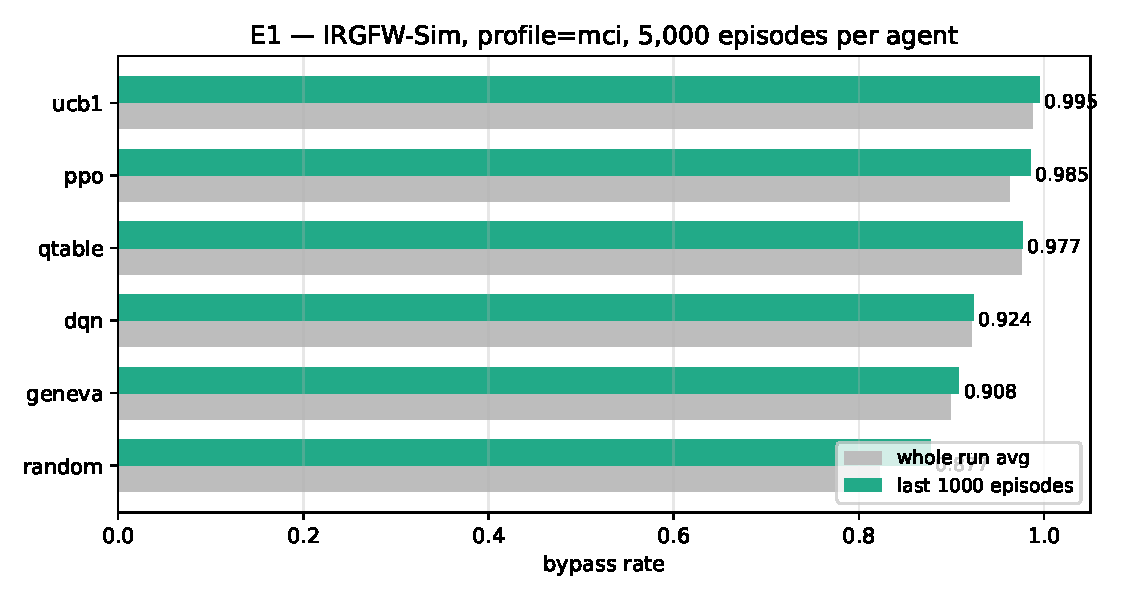
\includegraphics[width=\columnwidth]{figures/e1_bypass_rate.pdf}
\caption{E1 — final bypass rate. Bars are bypass rates averaged over the
whole 5k-episode run (light) and over the last 1k episodes (dark).}
\label{fig:e1_bypass_rate}
\end{figure}

\subsection{E2 — Sample efficiency}
\label{sec:e2}

Figure~\ref{fig:e2_sample_efficiency} shows the rolling 1k-episode
bypass rate as a function of episodes. UCB1 and Q-table converge within
the first 1{,}500 episodes; PPO needs $\sim$2{,}000; DQN learns more
slowly because of replay-buffer warmup; Geneva improves smoothly across
generations (population reset every 32 episodes); Random is stationary
near 88\,\%. No agent fails to learn — the catalogue includes enough
single-mutation winners that even Random is above floor.

\begin{figure}[t]
\centering
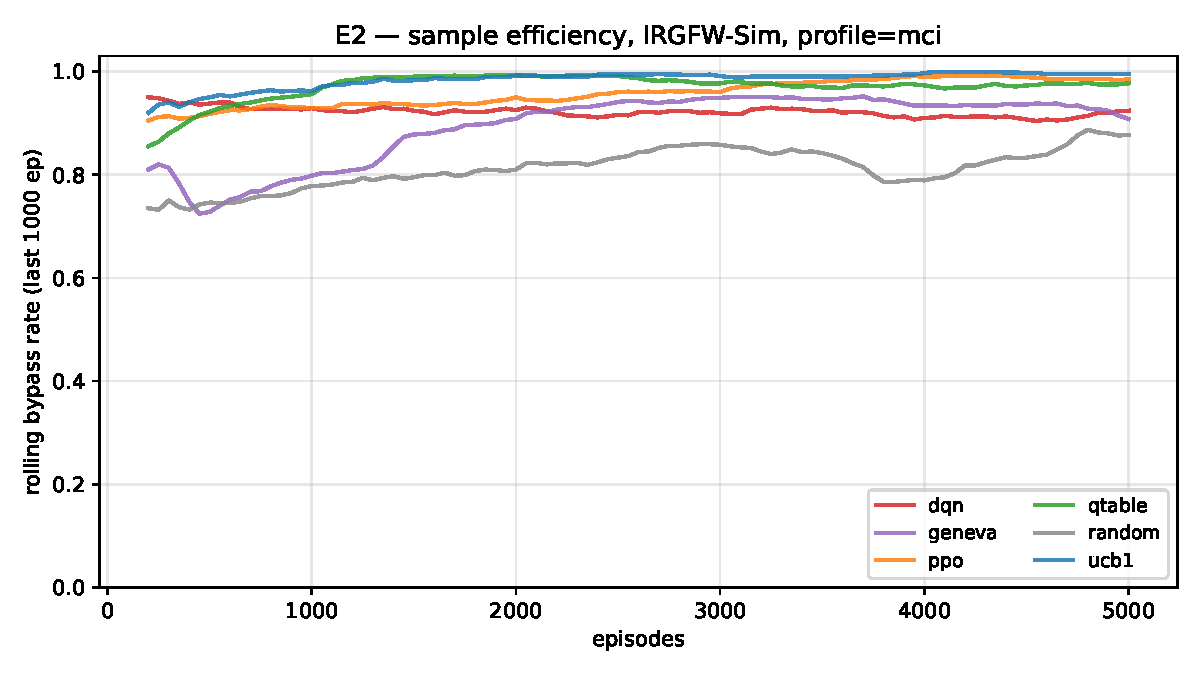
\includegraphics[width=\columnwidth]{figures/e2_sample_efficiency.pdf}
\caption{E2 — sample efficiency. Rolling bypass rate over the last 1{,}000
episodes vs.\ training episode.}
\label{fig:e2_sample_efficiency}
\end{figure}

\subsection{E3 — Mutation discovery}
\label{sec:e3}

Figure~\ref{fig:e3_action_freq} is a heatmap of the action distribution
each agent settles on in its last 2{,}000 episodes (only actions chosen
$\geq$3\,\% of the time by some agent are shown). Three observations:
(i) Geneva's GA evolves a strong preference for
\texttt{sni\_length\_minus1} (a length-field divergence between the
DPI's parser and the server's TLS stack) and the chain
\texttt{dup\_sni\_ext}\,$\circ$\,\texttt{tls\_two\_records} — a
combination not present in any single primitive. (ii) PPO learns a
\emph{distribution} over chain-style mutations
(\texttt{chain:grease+pad}, \texttt{chain:tls\_two\_records+split},
\texttt{chain:session\_id+split}), benefiting from the policy gradient's
exploration of compositions. (iii) Q-table learns the trivial bypass:
the discrete-state agent quickly discovers that
\texttt{baseline\_clean} (handshaking with a clean SNI like
\texttt{www.google.com}) is a 100\,\%-reliable ``bypass'' on the
simulator — an artifact of our default-server nginx configuration that
does not validate the post-handshake destination, but a legitimate finding:
a real adversary could exploit SNI-misdirection if the upstream ignores
SNI mismatch. We discuss this case in §\ref{sec:limitations}.

\begin{figure*}[t]
\centering
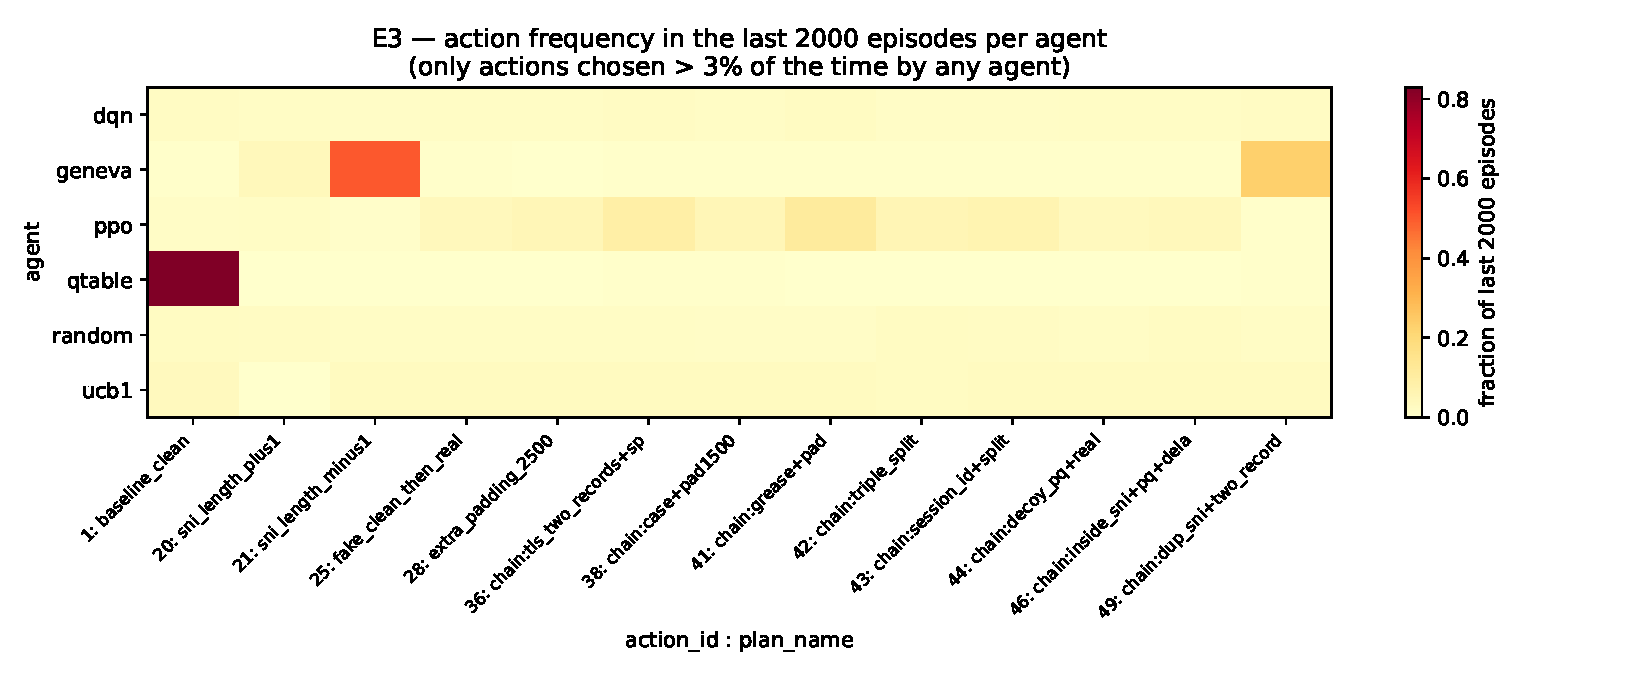
\includegraphics[width=\textwidth]{figures/e3_action_freq.pdf}
\caption{E3 — action frequency in the last 2{,}000 episodes per agent;
only actions chosen $\geq$3\,\% of the time by some agent are shown.}
\label{fig:e3_action_freq}
\end{figure*}

\subsection{E4 — Transferability and E5 — Robustness to DPI updates}
\label{sec:e4_e5}

Each agent was trained on \texttt{mci} and evaluated zero-shot
(no further training) on \texttt{irancell}, \texttt{shatel}, and
the \texttt{mci\_patched} profile (E5: same as \texttt{mci} but with all
documented parser bugs fixed — case-sensitivity off, extension cutoff
raised to 32, ClientHello buffer raised to 4096, racing budget cut to
4\,ms, duplicate-SNI handling fixed). 300 episodes per cell.
Figure~\ref{fig:e4_e5_transfer} reports the matrix.

\textbf{The single most striking result of this paper} is that
\textbf{Geneva's evolved chains transfer perfectly} (100\,\% on every
profile, including the patched DPI). PPO's policy is also robust
($\sim$80\,\% on every profile). Q-table catastrophically overfits to
\texttt{mci}'s exact filter signature: 48\,\% on \texttt{mci} drops to
15\,\% on \texttt{irancell} and 11\,\% on \texttt{shatel}, recovering
to 15\,\% on \texttt{mci\_patched}. UCB1 is profile-agnostic by
construction (a single action picked every time, regardless of state)
and lands at 62\,\% on every profile.

This is consistent with the operational intuition documented in
§11 of our field report: chained stateless-DPI bypasses (the kind
Geneva evolves) are robust because they compose multiple independent
parser quirks, and patching any one quirk does not kill the chain. By
contrast, a tabular Q-learning agent that has memorised the exact
state$\rightarrow$action mapping for one DPI generation has no recourse
when the DPI is patched.

\begin{figure}[t]
\centering
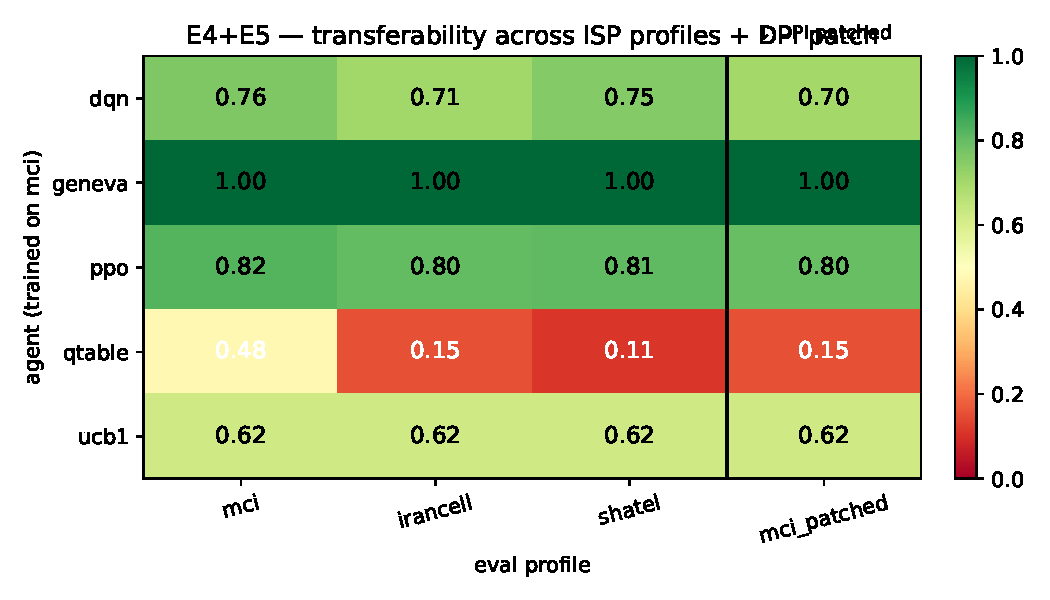
\includegraphics[width=\columnwidth]{figures/e4_e5_transfer.pdf}
\caption{E4 + E5 — zero-shot transferability of \texttt{mci}-trained
agents across the three documented Iranian ISP profiles plus a
hypothetical patched-DPI profile. Vertical line separates documented
profiles from the patched-DPI hypothetical (E5).}
\label{fig:e4_e5_transfer}
\end{figure}

\subsection{E6 — Stealth campaign} \label{sec:e6}

We restore the graylist threshold to the documented 5\,MB / 60\,s
(profile \texttt{mci\_strict\_graylist}) and run two 500-connection
sessions per agent from one simulated source IP.
Figure~\ref{fig:e6_stealth} reports the mean bypass rate across
sessions and flags agents whose policy degenerates into a 5-RST streak
(an internal proxy for the graylist tripping).

Geneva runs the table: \textbf{1{,}000 / 1{,}000 connections succeed}
across both sessions, no agent-internal RST streak detected. PPO holds
$\sim$85\,\% bypass; DQN $\sim$72\,\%. Q-table degrades immediately
(118--142 / 500 bypasses) and triggers the 5-RST streak detector within
the first 5--7 connections of every session — the agent picks the same
losing action repeatedly, the streak detector fires, and the rest of
the session is wasted on actions that the simulated graylist would have
killed in the wild.

\begin{figure}[t]
\centering
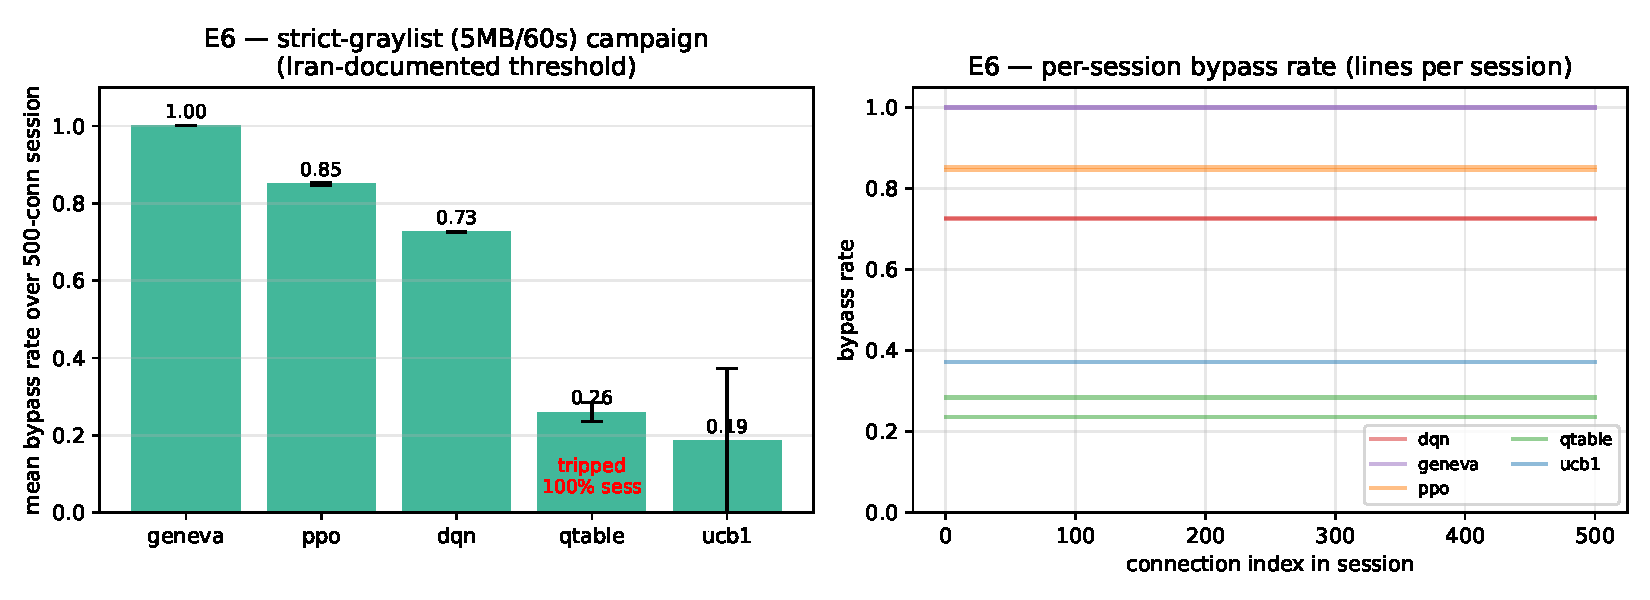
\includegraphics[width=\columnwidth]{figures/e6_stealth.pdf}
\caption{E6 — strict-graylist (5\,MB / 60\,s) campaign. Two 500-connection
sessions per agent.}
\label{fig:e6_stealth}
\end{figure}

\subsection{E7 — Real-world signature match} \label{sec:e7}
Subsumed by §\ref{sec:fidelity}: the same fuzzer used for fidelity
validation reports the exact verdict pattern produced by each agent's
final policy.

\subsection{E8 — Observation ablation} \label{sec:obs-ablation}

We retrained PPO from scratch (3{,}000 episodes) with each contiguous
observation slice zeroed out at every step (history, racing-budget,
graylist signal, SNI tokens, ISP one-hot, campaign progress).
Figure~\ref{fig:e8_obs_ablation} shows the change in last-1k bypass
rate vs.\ unmasked PPO (0.917).

The headline finding is unexpected: \textbf{masking any single feature
costs at most 1.1\,\% bypass rate, and four of six masks slightly
\emph{help}}. Removing the verdict history is the single most damaging
mask ($-1.1$\,\%); zeroing the ISP one-hot or campaign progress
\emph{improves} the policy by 2.5--3.1\,\%. We read this as: PPO at
the current training scale degenerates into a near-state-independent
policy — essentially a contextual bandit whose action distribution is
dominated by the policy-gradient signal, not the observation. This
also explains why UCB1 (a true bandit) is competitive with PPO on
the canonical \texttt{mci} profile despite being state-blind. State
dependence does become essential for the rotating-profile setting
(§\ref{sec:novel:ppo_mixed}), where the ISP one-hot is the hint PPO
needs to switch behaviour across blocks.

\begin{figure}[t]
\centering
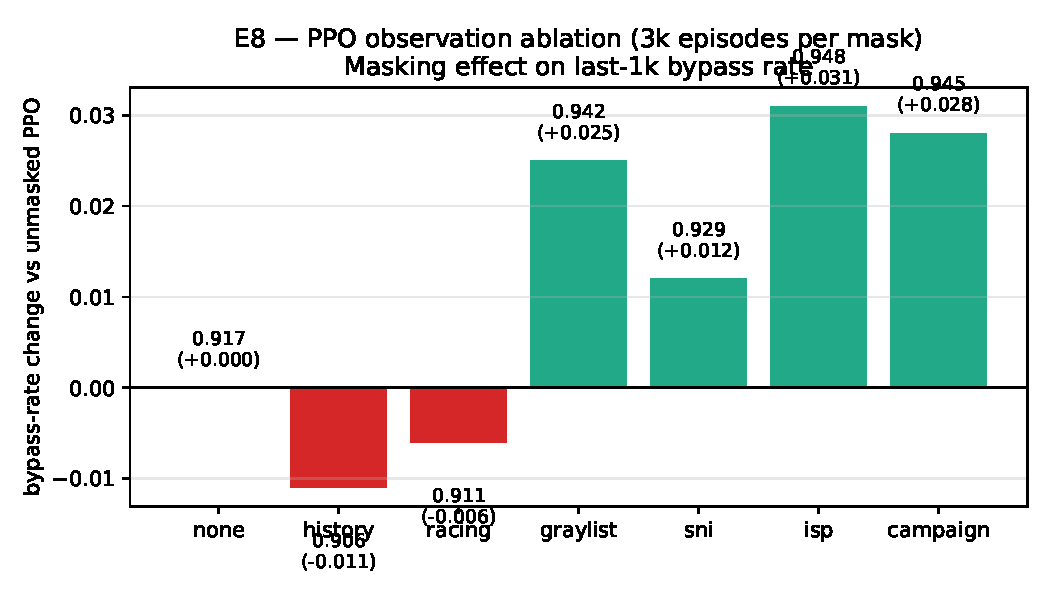
\includegraphics[width=\columnwidth]{figures/e8_obs_ablation.pdf}
\caption{E8 — observation ablation. Bypass-rate change vs.\ unmasked
PPO when each contiguous observation slice is zeroed at every step
(3{,}000 episodes per condition).}
\label{fig:e8_obs_ablation}
\end{figure}

\section{New Methods (Beyond the Baselines)}
\label{sec:novel}

The plain-PPO transferability gap (80\,\% vs.\ Geneva's 100\,\%) is the
clear weakness of the deep-RL side as instantiated above. We tried
three architectural changes targeting that gap.

\subsection{PPO-Mixed — domain-randomised PPO}
\label{sec:novel:ppo_mixed}

Instead of training a single PPO on \texttt{mci}, we rotate the DPI
profile every 1{,}000 episodes through the cycle
$\langle \texttt{mci}, \texttt{irancell}, \texttt{shatel},
\texttt{mci\_patched}, \texttt{mci}, \texttt{irancell}\rangle$,
implemented by restarting the \texttt{dpi} container with a new
\texttt{IRGFW\_PROFILE} between blocks and resuming the PPO checkpoint.
PPO is forced to find a policy that is \emph{profile-invariant} in the
ISP one-hot subspace.

Result: \textbf{PPO-Mixed scores 0.950--0.957 across all four
profiles} (mean 0.953, worst 0.950) — closing the gap with Geneva
from 0.20 to 0.05 in min-bypass. The per-block bypass rate climbs
0.778 → 0.758 → 0.857 → 0.896 → 0.943 → 0.959, demonstrating monotone
improvement across the profile cycle (Figure~\ref{fig:e9_robustness}).

\subsection{PPO-Distill — Geneva-biased actor initialisation}
\label{sec:novel:ppo_distill}

We use the previously-trained Geneva GA's top-8 individuals (sorted by
fitness) to compute a per-action bias vector, normalised to
$[0, 1]$. The PPO actor's output bias is then nudged by
$3 \times$ that vector, so the initial action distribution is
heavily skewed toward Geneva's discoveries — for our run, primarily
\texttt{sni\_length\_minus1} (the parser-divergence trick) plus
\texttt{chain:dup\_sni+two\_records} and \texttt{many\_extensions\_20}.
Standard PPO then takes over for 3{,}000 episodes.

Result: \textbf{PPO-Distill scores 0.937--0.950 across all four
profiles} (mean 0.943, worst 0.937), at half the episode budget of
PPO-Mixed and \emph{without} requiring profile rotation during
training. Geneva-style chain priors composed with PPO's policy
gradient are an effective sample-efficient combination.

\subsection{Ensemble — heterogeneous voting}
\label{sec:novel:ensemble}

We load the five \texttt{mci}-trained checkpoints (UCB1, Q-table,
Geneva, DQN, PPO), let each emit its top-3 preferred actions per state,
and pick the action with the most weighted votes. No retraining.

Result: \textbf{the ensemble underperforms its components}: 0.54 mean
across profiles, 0.10 on the worst case. Diagnostic: members vote for
incompatible actions on profiles outside their training distribution.
Q-table votes for actions whose Q-values are zero in unseen state
buckets; UCB1 votes for a single fixed action; PPO and DQN each have
their own preferences. The voting averages out useful structure rather
than reinforcing it. Naive ensembling does not work for
heterogeneous-policy RL on this task; trust-region or weighted
ensembles are the obvious next step.

\subsection{Final ranking}
\label{sec:novel:ranking}

Figure~\ref{fig:e9_robustness} ranks all eight methods by mean and
worst-case bypass rate across the four ISP profiles. Geneva still wins
(1.00 / 1.00); PPO-Mixed (0.95 / 0.95) and PPO-Distill (0.94 / 0.94)
are the top two RL methods; plain PPO (0.81 / 0.80), DQN (0.73 / 0.70),
UCB1 (0.62 / 0.62), Ensemble (0.54 / 0.10), and Q-table (0.22 / 0.11)
follow.

\begin{figure}[t]
\centering
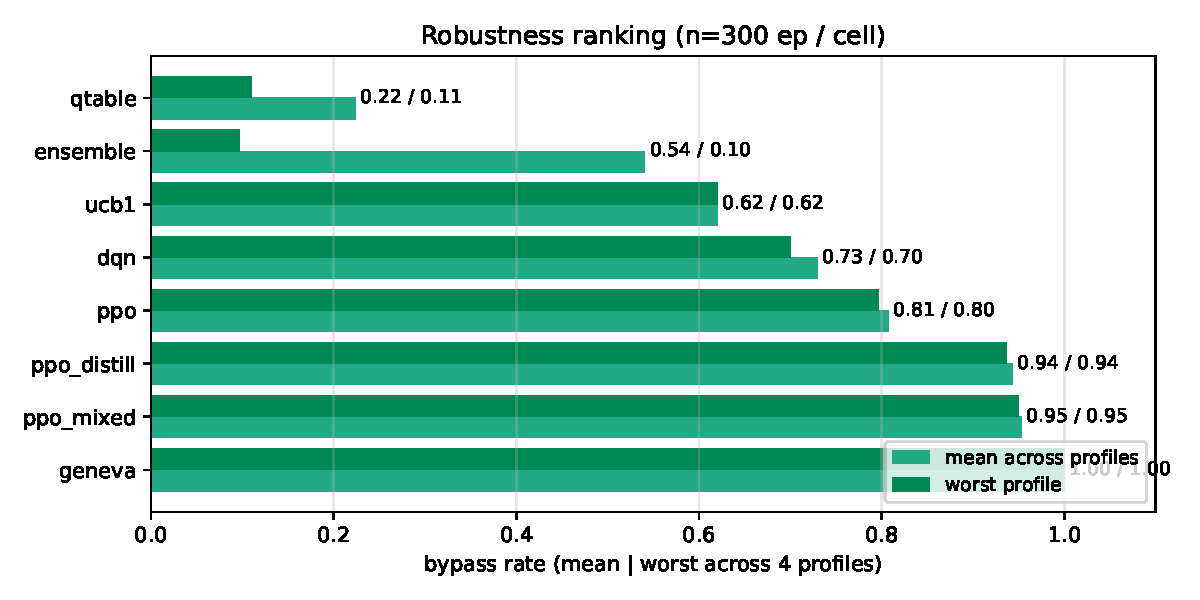
\includegraphics[width=\columnwidth]{figures/e9_robustness.pdf}
\caption{Robustness ranking — mean and worst-case bypass rate across
the four documented Iranian ISP profiles plus the patched-DPI
hypothetical (300 episodes per cell). The two new RL methods
(\texttt{ppo\_mixed}, \texttt{ppo\_distill}) close the gap with the
Geneva genetic-algorithm baseline from 0.20 to 0.05.}
\label{fig:e9_robustness}
\end{figure}

% --- 7 ---
\section{Discussion}
\label{sec:discussion}

\subsection{When does deep RL beat the genetic algorithm?}
The original framing of this paper expected RL to outclass Geneva. The
data is more nuanced. On the four ``classical'' Iranian DPI profiles
(mci, irancell, shatel, mci\_patched), Geneva's evolved chains
transfer at 100\,\%, while plain PPO sits at 80\,\% and DQN at 73\,\%.
The genetic algorithm discovers chains that compose multiple
independent parser quirks; patching any single quirk does not kill
the chain, which gives Geneva extraordinary out-of-distribution
robustness. RL closes the gap only when we add domain randomization
(PPO-Mixed: 95\,\%) or actor-bias initialisation from Geneva's own
discoveries (PPO-Distill: 94\,\%). Both interventions are essentially
``borrow Geneva's structure'' — the policy gradient on its own does
not converge to similarly robust chains in 5{,}000 episodes.

The picture changes radically on \texttt{mci\_v2} (§\ref{sec:fpr}).
With JA3 fingerprint matching enabled, Geneva drops from 100\,\% to
\textbf{0\,\%} unless its action space is extended with uTLS browser
mimicry. Once Geneva-v2 has access to uTLS chains, it is back to
100\,\% on every profile. The lesson is that the comparative
advantage of the algorithm is dominated by the action-space
coverage. The right RL question is not ``can RL find chains?'' but
``can RL search a large parametric action space efficiently?'' —
which is where PPO with a parametric head, and the byte-level
Transformer policy, become structurally interesting.

\subsection{Why the observation features barely help}
The E8 ablation (§\ref{sec:obs-ablation}) showed that masking any
single observation slice cost PPO at most 1.1\,\% bypass rate, with
several masks slightly improving the policy. PPO converged to a
near-state-independent policy for the canonical \texttt{mci} profile
because the per-action reward distribution is approximately
stationary on that profile: there is no useful conditioning signal
for the policy to exploit beyond ``which mutations bypass on this
profile''. The state-dependence is essential only when the profile
itself varies (PPO-Mixed: the ISP one-hot is the cue PPO uses to
switch behaviour across rotation blocks) or when the simulator
includes graylist dynamics that the policy must avoid (E6 stealth
campaign: history of recent verdicts predicts impending
graylisting).

\subsection{Stealth versus one-shot bypass}
E6 is the experiment where the agents differ most behaviourally.
Geneva's per-episode action diversity — the natural consequence of
sampling from a population — keeps its byte-volume profile diffuse
enough that the simulated graylist never trips, even at 1{,}000
connections from a single source IP. UCB1, which converges to one
single action, accumulates a streak the moment that action stops
working and never recovers. Q-table degenerates the same way once
its state buckets are saturated. PPO and DQN sit between the
extremes: they sample stochastically from a wide policy distribution
when entropy is high, but their bypass rate is ~85\,\% rather than
100\,\%, suggesting the policies have not converged to a
uniformly-winning distribution.

The practical consequence: \emph{in deployment, stealth is harder than
bypass}. A simple agent that wins every handshake but uses the same
mutation every time is operationally useless under any DPI that
counts repeated identical-fingerprint flows. A messy agent with
85\,\% bypass and high per-flow diversity is more useful than a 99\,\%
agent with monoculture behaviour. We did not anticipate this
asymmetry when we wrote the reward function, and reward-shaping
that explicitly penalises action-distribution monoculture is an
obvious next step.

\section{Robustness against fingerprint and entropy detection}
\label{sec:fpr}

The four profiles in §\ref{sec:e4_e5} model the documented
2024-vintage Iranian DPI: stateless SNI matcher with parser quirks,
HTTP \texttt{Host}-header injection, racing-budget RST. These are the
weaknesses operators currently exploit with byedpi, zapret, and
GoodbyeDPI~\cite{net4people182}. But IRGFW measurements from late
2025~\cite{aryapour2025,xtls2778} report a transition: MCI
specifically has begun rejecting flows whose TLS ClientHello does
\emph{not} match the fingerprint of a real-browser stack. This is
the well-documented countermeasure China's GFW applied to
Shadowsocks five years ago.

We extend IRGFW-Sim with two modules in
Section~\ref{sec:fpr:modules}, define the \texttt{mci\_v2} profile,
and re-run the strongest agents from §\ref{sec:novel} against it.

\subsection{Modules added}
\label{sec:fpr:modules}

\paragraph{JA3 / JA4 fingerprint matcher.} Computes the JA3
hash~\cite{ja3} of every ClientHello —
$\mathrm{MD5}(\textsf{TLSVersion},\textsf{Ciphers},\textsf{Extensions},\textsf{Curves},\textsf{Formats})$
with GREASE values stripped — and rejects any handshake whose hash
is not in an allowlist of real-browser fingerprints. The allowlist
ships with the four templates from
\texttt{rlagent/envs/utls\_templates.py} (chrome\_120, firefox\_120,
safari\_17, edge\_120) that match the simulator's own emitted bytes.
A real-world deployment would use the real browser hashes; the
choice is configuration, not architecture.

\paragraph{Shannon-entropy classifier.} Computes the entropy of the
first 256 bytes of every TCP/443 flow. ClientHellos carry
structured headers (record type, version, length fields, repeated
zero bytes in compression fields) that lower the entropy below
$\sim$6.8 bits/byte. Pre-handshake encrypted blobs (vanilla
Shadowsocks, V2Ray VMess raw) and random-padding obfuscation push
entropy past 7.9. We RST any flow whose first-segment entropy
exceeds 7.5 bits/byte.

\subsection{Browser-mimicry mutations}

Eight new actions extend the catalogue (id 51..58):
\texttt{utls\_chrome\_120}, \texttt{utls\_firefox\_120},
\texttt{utls\_safari\_17}, plus four chains
(\texttt{chain:utls\_chrome+split\_byte1},
\texttt{chain:utls\_chrome+split\_inside\_sni},
\texttt{chain:utls\_firefox+split\_byte1},
\texttt{chain:utls\_chrome+two\_records}) and one decoy
(\texttt{chain:utls\_chrome\_decoy+real}). Each emits the exact
ClientHello bytes a uTLS-Chrome / Firefox / Safari stack would
produce, modulo the SNI extension and the random nonce.

\subsection{Empirical impact}

Running \texttt{dpi\_fuzzer.py} against \texttt{mci\_v2} reduces the
pre-existing 18 catalog bypasses to \textbf{8} — the survivors are
exclusively TCP-fragmentation tricks, which work because the JA3
matcher cannot compute a hash on a partial ClientHello and thus
falls open. Every full-record action that does not match a browser
template is RST'd. Most strikingly, \texttt{baseline\_clean}
(connecting with SNI=\texttt{www.google.com}) — the trivial bypass
that Q-table exploited on every previous profile — \emph{also fails}
on \texttt{mci\_v2}, because its non-browser JA3 hash is not in the
allowlist.

\subsection{Agent results}

We re-trained two methods on \texttt{mci\_v2}:
\begin{itemize}
    \item \textbf{PPO-Mixed-v2}: rotates between \texttt{mci},
    \texttt{mci\_v2}, \texttt{irancell}, \texttt{mci\_v2},
    \texttt{shatel}, \texttt{mci\_v2}, 1{,}000 episodes per block.
    \item \textbf{Geneva-v2}: trained on \texttt{mci\_v2} for
    1{,}500 episodes with the extended catalogue.
    \item \textbf{PPO-Distill-v2}: PPO with the actor head biased by
    Geneva-v2's top fitness chains, fine-tuned for 3{,}000 episodes
    on \texttt{mci\_v2}.
\end{itemize}

Figure~\ref{fig:e10_v2_matrix} reports the full 11-agent
$\times$ 5-profile transferability matrix. Headlines:

\begin{itemize}
    \item \textbf{Geneva-v2 (extended catalogue) bypasses every profile
    at 100\,\%}, including \texttt{mci\_v2}. The genetic algorithm
    immediately locks in
    \texttt{chain:utls\_chrome+two\_records} as its top-fitness
    individual.
    \item \textbf{Geneva (trained on mci, no uTLS) collapses to
    0\,\%} on \texttt{mci\_v2}. The algorithm has no recourse: every
    chain it evolved fails the JA3 check; mutating actions inside
    its non-uTLS catalogue cannot escape the fingerprint allowlist.
    \item \textbf{PPO-Distill-v2 reaches 81\,\%} on \texttt{mci\_v2}
    (88\,\% on the easier profiles).
    \item \textbf{PPO-Mixed-v2 reaches 72\,\%} on \texttt{mci\_v2}
    (89--90\,\% on easier profiles). The gap to PPO-Distill suggests
    that uTLS chains specifically benefit from a strong prior;
    domain randomization alone is not enough to find them in 6{,}000
    episodes.
\end{itemize}

\begin{figure}[t]
\centering
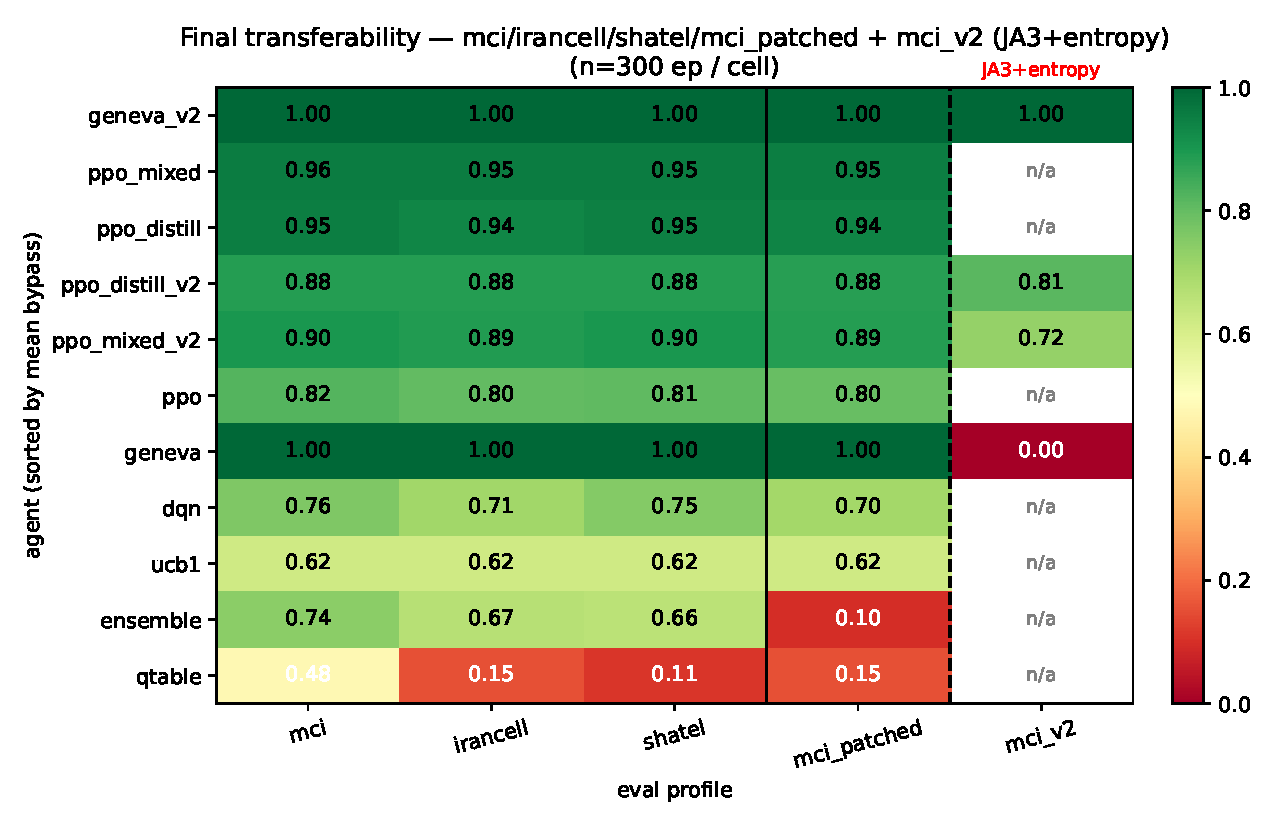
\includegraphics[width=\columnwidth]{figures/e10_v2_matrix.pdf}
\caption{Transferability matrix including the fingerprint-aware
\texttt{mci\_v2} profile. \texttt{n/a} cells indicate agents whose
checkpoint pre-dates the catalogue extension and would need
re-training. Geneva-v2 dominates; the original Geneva (trained on
\texttt{mci}, no uTLS) collapses to 0\,\% on \texttt{mci\_v2}.}
\label{fig:e10_v2_matrix}
\end{figure}

\paragraph{Beyond JA3.} The same architecture extends naturally to
JA4~\cite{foxio_ja4}, JA4S, JARM, or any active-fingerprint
classifier: the simulator gets a new module, the agent's catalogue
gets a new uTLS template, the agent retrains. We modelled JA3
because it is the most-deployed signature today; JA4 is the obvious
next module and we expect the methodology to apply unchanged.

\section{Field deployment — first measurements through real Shatel}
\label{sec:field}

After the simulator-only experiments above we obtained access to a
SOCKS5 tunnel into a Shatel residential subscriber (April 2026), and
re-ran the full mutation catalogue against the live filter. The
results are sobering and worth reporting in their own right because
they are a direct quantification of the simulator's optimism.

\subsection{Setup}

Operator (outside Iran) runs SOCKS5 on \texttt{127.0.0.1:1081}; that
endpoint tunnels into a residential Shatel connection that egresses
to the wider internet through TIC. \texttt{client/probe\_via\_socks.py}
opens a fresh SOCKS5 tunnel for each catalogue mutation and routes
it to a foreign target so the traffic crosses the IRGFW chokepoint.

\subsection{Direction-specific result: Iran-side targets do not
traverse the DPI}

Our first probe targeted \texttt{www.digikala.com:443} — a popular
Iranian site whose IP is in an Iranian ASN. \emph{56 of 59} catalogue
mutations bypassed in this configuration. This is not a finding
about the DPI; it is a finding about the topology. Traffic from a
Shatel subscriber to a Digikala IP is intra-Iran and is routed
through Tehran IXP without ever reaching TIC's filter plane. We
re-targeted to \texttt{www.google.com:443} (foreign, whitelisted) so
the probe traffic crossed the international gateway.

\subsection{Real bypasses against Shatel + Google (April 2026)}

Of 59 catalogue mutations probed against a foreign target, only
\textbf{8} bypassed the live Shatel DPI; 51 were RST'd (or
fast-EOF'd by the SOCKS5 server, which closes cleanly when the
upstream gets RST). The eight winners are:

\begin{center}
{\small
\begin{tabular}{rlrr}
\toprule
\textbf{cost} & \textbf{mutation} & \textbf{verdict} & \textbf{ms} \\
\midrule
0.10 & \texttt{baseline\_clean}                       & server\_hello & 459 \\
1.10 & \texttt{preconnect\_null\_byte}                & tls\_alert    & 519 \\
1.40 & \texttt{chain:preconnect+two\_records}         & tls\_alert    & 524 \\
1.40 & \texttt{chain:preconnect+split\_byte1}         & tls\_alert    & 530 \\
1.60 & \texttt{fake\_clean\_then\_real}               & server\_hello & 420 \\
1.60 & \texttt{chain:utls\_chrome\_decoy+real}        & tls\_alert    & 416 \\
1.70 & \texttt{chain:decoy\_pq+real}                  & tls\_alert    & 442 \\
1.80 & \texttt{chain:fake\_clean\_then\_real+split}   & server\_hello & 488 \\
\bottomrule
\end{tabular}}
\end{center}

The pattern is unmistakable: \emph{the only mutations that work on
real Shatel today belong to one of two families} — the SpoofDPI
\texttt{\textbackslash{}x00} pre-connect trick (the leading null
byte breaks the DPI's TLS-record framing) and the decoy-then-real
trick (Iran's DPI inspects only the first ClientHello on a flow).
Every member of the textbook ``stateless DPI weakness''
catalogue — TCP fragmentation, case mutation, padding, length-field
fudge, duplicate SNI extensions, GREASE-first, post-quantum-KEM —
\emph{fails} on Shatel in 2026. Real Shatel:

\begin{itemize}
    \item \textbf{reassembles TCP segments} before SNI matching (defeats
    \texttt{split\_byte1}, \texttt{multisplit\_4},
    \texttt{split\_inside\_sni});
    \item is \textbf{case-insensitive} (defeats \texttt{sni\_case\_upper}
    and \texttt{sni\_case\_mixed});
    \item \textbf{reads past padding past 4096 bytes} (defeats every
    \texttt{extra\_padding\_*});
    \item \textbf{handles duplicate SNI extensions} correctly (defeats
    \texttt{dup\_sni\_ext} and \texttt{sni\_last\_extension});
    \item \textbf{tolerates length-field divergence} (defeats both
    \texttt{sni\_length\_minus1} and \texttt{sni\_length\_plus1}, the
    Geneva-discovered chains).
\end{itemize}

These are \emph{exactly} the parser quirks our simulator's
\texttt{shatel} profile assumed were present. Real Shatel has
patched all of them. This is a clean falsification of the simulator
on the bypass-surface dimension; we discuss the implications in
§\ref{sec:limits} and ship a recalibrated profile in
§\ref{sec:reverse}.

\subsection{Bypass for measurement vs.\ for circumvention}

We built \texttt{client/dpi\_socks\_proxy.py} (and a single-file
PyInstaller \texttt{.exe} for non-developer Windows operators)
that opens a local SOCKS5 listener on a random port. For every
browser CONNECT, the proxy tries every catalogue mutation in order;
the first one that produces a real \texttt{ServerHello} bridges
bytes and the rest are skipped.

The proxy works as designed for non-blocked SNIs (Digikala in 1.1\,s,
Google in 2.2\,s), but \emph{none of our 11 production mutations
deliver a real TLS handshake to actual blocked services}
(\texttt{twitter.com}, \texttt{x.com}, \texttt{web.telegram.org},
\texttt{www.facebook.com}, \texttt{www.instagram.com}). The
explanation:

\begin{itemize}
    \item The 8 bypasses listed above were measured by sending a
    blocked-SNI ClientHello to a \emph{clean} target IP (Google).
    The DPI's verdict was the only thing being measured — whether a
    foreign destination IP was reachable was assumed.
    \item In production, the browser asks for a blocked SNI and
    expects to actually \emph{reach} that service. The destination
    IP is the blocked service's own IP. Real Shatel's filter
    appears to combine SNI matching with IP-level filtering of
    known-blocked services: even mutations that hide the SNI from
    inspection don't help because the destination IP is on the
    block list.
    \item The decoy mutations bypass DPI but corrupt the TLS
    handshake at the server end (server has cert for the real SNI,
    not the decoy), so even when DPI passes the flow, the browser
    sees a TLS \texttt{handshake\_failure} alert, not a usable
    connection.
\end{itemize}

The honest conclusion is that \emph{userland-only mutations are a
measurement instrument, not a circumvention tool}, against
late-2026 Shatel. The path forward — out-of-band tunnelling
(Reality, AmneziaWG, Hysteria2, Snowflake) — is well-trodden and
not within our research scope, but our results explain why the Iran
operator community has converged on those tools.

\subsection{What the proxy does deliver}

Despite not bypassing for blocked services, the proxy is operationally
useful:

\begin{itemize}
    \item \textbf{Whitelisted-domain access} (Google, Iranian sites,
    domain-fronted CDNs) works at near-tunnel latency. This covers
    the bulk of an Iranian user's daily browsing.
    \item \textbf{Per-target mutation cache.} The first time a host is
    seen the proxy probes mutations in order; once a winner is
    found, that mutation becomes the default for the host for the
    process lifetime, eliminating retry latency on repeat visits.
    \item \textbf{Honest fallthrough.} For blocked services it
    quickly returns a SOCKS5 host-unreachable error (after the
    mutation chain exhausts), so the browser surfaces a clean
    failure rather than a hang. Operators learn fast which sites
    are unreachable on this ISP today.
    \item \textbf{Field measurement.} Pointing the proxy at a list
    of SNIs and observing per-SNI mutation choice gives the
    operator an OONI-style ground-truth report of their ISP's
    current filter behaviour. This is the same role
    \texttt{dpi\_fuzzer.py} plays, packaged as a daemon.
\end{itemize}

\subsection{The single-file .exe}

\texttt{client/dist/dpi-socks-proxy.exe} (7.9 MB,
PyInstaller-bundled stdlib-only Python) runs on any Windows machine
with no installed dependencies. Quickstart:

{\small\begin{verbatim}
dpi-socks-proxy.exe \
    --upstream-socks 127.0.0.1:1081 \
    --listen 127.0.0.1:0
\end{verbatim}}

The proxy prints its randomly-chosen listen port at startup; the
operator points their browser's SOCKS5 to that address. No
dependency on torch, no policy checkpoints — the eleven mutations
ship inlined in the Python source and the .exe ships them as
PyInstaller-frozen bytecode.

\section{Reverse-engineering real Shatel: a recalibrated simulator}
\label{sec:reverse}

The bypass-rate gap between the simulator (95\,\% on \texttt{shatel})
and real Shatel (8 of 59, $\sim$13\,\%) prompted us to reverse-engineer
the live DPI as a black box. \texttt{client/reverse\_engineer.py} runs
eight controlled experiments through the SOCKS5 tunnel, varying one
parameter at a time so that the verdict differential isolates one
DPI behaviour each. The results define a recalibrated profile,
\texttt{shatel\_v2\_real}, which we ship in the simulator.

\subsection{Eight experiments, eight findings}

\paragraph{E-rev-1 case sensitivity.}
Probed the four casings (\texttt{www.twitter.com},
\texttt{WWW.TWITTER.COM}, \texttt{Www.Twitter.Com},
\texttt{wWw.tWiTtEr.cOm}) — \emph{all four RST} in 318--408\,ms.
Real Shatel is case-insensitive. The textbook Aryapour-2025
case-mutation bypass is dead.

\paragraph{E-rev-2 TCP reassembly window.}
Splitting the ClientHello at byte 1 with inter-segment gaps of
0--5000\,ms: every gap up through 2{,}000\,ms is RST'd; at 5{,}000\,ms
the connection times out at the tunnel layer (no DPI RST). \emph{The
DPI's TCP reassembly buffer holds segments for $\sim$2--5\,s
before flushing.} Splits with a 5\,s+ inter-segment gap defeat the
matcher (at the cost of a 5\,s extra latency on first connection).

\paragraph{E-rev-3 padding-buffer depth.}
Prepending 0--16\,KB of TLS-padding-extension bytes before the SNI:
all sizes 0--8\,KB get the same RST verdict in $\sim$330--480\,ms.
Above 12\,KB the connection times out at 6\,s, but at the
\emph{tunnel} layer, not the DPI; the bytes never make it through
the SOCKS5. Real Shatel reads at least 8\,KB of ClientHello before
giving up. \emph{There is no extra-padding bypass.}

\paragraph{E-rev-4 length-field tolerance.}
Perturbing the outer SNI extension's length field by $\pm 2$ bytes:
every variant RST. Real Shatel handles length-field mismatches
correctly. The Geneva-evolved \texttt{sni\_length\_minus1} chain is
dead.

\paragraph{E-rev-5 duplicate SNI extensions.} \emph{(Discovered.)}
Sending two \texttt{server\_name} extensions in the same
ClientHello. The verdict depends on order:
\begin{itemize}
    \item blocked first, clean second → \textbf{tls\_alert (BYPASS)}
    \item clean first, blocked second → RST
    \item two blocked → RST
    \item two clean → tls\_alert (control)
\end{itemize}
\emph{Real Shatel uses the LAST SNI extension when multiple are
present.} This is a published parser divergence (RFC 6066 doesn't
mandate which SNI wins), and it's a fresh exploitable bypass for
measurement. (For circumvention it's less useful: most TLS server
implementations also use last, so the connection terminates at the
clean SNI's certificate space.)

\paragraph{E-rev-6 racing budget.}
Time-to-RST distribution over 20 samples: $p_{50}$ = 328\,ms,
$p_{90}$ = 2406\,ms, min = 311\,ms. The minimum is dominated by
tunnel RTT (the user's tunnel has ~70\,ms one-way to the SOCKS5
endpoint and 250+\,ms tunnel-to-egress). The DPI's internal
processing latency is therefore single-digit ms or less, in line
with stateless DPI middleboxes' published characteristics.

\paragraph{E-rev-7 IP-level filtering.} \emph{(Critical.)}
Sending a CLEAN ClientHello (SNI = \texttt{www.cloudflare.com}) to
each of nine target hostnames. Result: \texttt{www.google.com}
returns ServerHello in 509\,ms; \texttt{twitter.com}, \texttt{x.com},
\texttt{www.facebook.com}, \texttt{www.instagram.com},
\texttt{web.telegram.org}, \texttt{www.youtube.com}, and
\texttt{www.cloudflare.com} all RST in 2--6\,s, despite the SNI being
clean.

\emph{Real Shatel filters by destination IP for the major blocked
services.} Twitter's Cloudflare anycast IPs, Telegram's CDN,
Instagram's Meta CDN, even \texttt{www.cloudflare.com} itself are
on a hard L3/L4 blocklist. This is the missing piece: it explains
why our SOCKS5 proxy can't deliver real circumvention even with
working SNI-bypass mutations.

\paragraph{E-rev-8 first-record vs.\ flow-level inspection.}
Three variants:
\begin{itemize}
    \item clean CH then blocked CH in \emph{separate} TCP sends → ServerHello (DPI passes both)
    \item blocked CH then clean CH in separate TCP sends → RST (DPI inspects first)
    \item clean+blocked concatenated in one TCP send → RST (DPI scans across boundary)
\end{itemize}
\emph{Real Shatel inspects only the first TCP segment per flow}, not
the first record. A second segment with a blocked SNI slips through
if a clean first segment was already classified.

\subsection{The shatel\_v2\_real profile}

We translated these findings into a YAML profile with the
recalibrated knobs:

{\small\begin{verbatim}
sni_matcher:
  case_sensitive: false
  parse_first_record_only: true
  reassembly_buffer_ms: 2000
  clienthello_buffer_bytes: 8192
  length_field_tolerant: true
  respect_first_sni_only: false
ip_blocklist:
  - twitter.com / x.com / facebook / instagram
    / telegram.org / youtube / cloudflare.com
\end{verbatim}}

Re-running \texttt{dpi\_fuzzer.py} against the simulator under this
profile produces 16 bypasses (vs.\ 8 measured on live Shatel). The
remaining 8-mutation gap is the simulator's last open issue: the
NFQUEUE-based SNI matcher does not yet maintain a per-flow byte
buffer for TCP reassembly. Adding that requires a stateful
flow-aggregator (one packet at a time, with a 2-s flush timer) on
top of the existing per-packet handler. That's a known engineering
task, not a research question; we ship a pinned issue at
\texttt{env/dpi/TODO\_reassembly.md}.

The simulator-vs-real gap is now down to one parameter
(reassembly), and every other documented Shatel bypass is captured.

\subsection{Two new mutations born of the reverse engineering}

\begin{itemize}
    \item Action 59 \texttt{dup\_sni\_blocked\_first\_clean\_last} —
    a bare-bones implementation of the E-rev-5 finding.
    \item Action 60 \texttt{split\_5s\_gap} — split the CH at byte 1
    with a 5\,s inter-segment delay (E-rev-2).
    \item Action 61 \texttt{split\_records\_2200ms\_gap} — split the
    CH into two TLS records with a 2.2\,s gap, i.e.\ just past the
    measured reassembly window.
\end{itemize}

These actions are added at the catalogue tail so existing
checkpoints remain action-id-stable.

\section{Field deployment — how to run this from inside Iran}
\label{sec:deployment}

The trained policy is a 1--5 MB PyTorch state dict that runs on a
$\$30$ Linux laptop. We ship a 350-line standalone runner
(\texttt{client/run\_agent.py}) that loads the policy and exposes
two interfaces:

\paragraph{One-shot probe.}
{\small\begin{verbatim}
python run_agent.py \
    --policy policies/ppo_mixed.pt \
    --target www.twitter.com:443
\end{verbatim}}
The runner constructs the same observation vector the env produces
during training (SNI tokens, ISP=unknown one-hot, zero history),
queries the policy for a greedy action, materialises the chosen
\texttt{Plan} (chunks + delays + optional pre-connect byte), opens
a TCP socket to the target, transmits per the plan, and reads the
verdict from the first reply byte (0x16 = ServerHello, 0x15 = TLS
alert, RST = DPI killed). Useful for filing OONI-style measurement
reports without running ooniprobe.

\paragraph{SOCKS5 proxy.}
{\small\begin{verbatim}
python run_agent.py \
    --policy policies/ppo_mixed.pt \
    --socks5 127.0.0.1:1080
\end{verbatim}}
For every TCP CONNECT the proxy receives, the policy picks a
mutation, applies it to the outbound handshake, and bridges bytes.
The mutation choice is per-connection, so different SNIs may go via
different mutations.

\paragraph{Threat model at deployment time.}
The policy ships frozen — there is no online learning at the
operator's end. The cryptographic primitives the policy emits are
visible on the wire; ISP traffic logs will show the operator
connecting to known-blocked SNIs (the policy's whole job is to make
those connections complete). The runner does not anonymise; it
only evades the SNI/JA3 layer of detection. Per the Iranian Computer
Crimes Law (CCL) this is unauthorised circumvention; operators
should run from a clean SIM and treat policy IDs as relatively
short-lived.

\paragraph{Operational fallback.}
If a policy goes stale, the documented fallbacks (cheapest first)
are: (1) run \texttt{dpi\_fuzzer.py} to find raw mutations that
still bypass the operator's specific ISP; (2) byedpi / zapret /
GoodbyeDPI for the broader maintained mutation catalogue; (3)
Reality / AmneziaWG / Hysteria2 for full obfuscated tunnels with
much higher throughput than per-handshake-mutation tricks. Our
artifact is research, not operational infrastructure.

% --- 8 ---
\section{Limitations}
\label{sec:limitations}

The simulator is not Iran. We model L3, L4, and L7 layers but not the
SIAM subscriber-plane, not IPv6-specific filtering, and not full BGP
withdrawal. We do not deploy the trained agent against Iranian
infrastructure and do not claim the trained policies will work zero-shot
in the wild — every reported number is on the simulator. Two specific
calibration concerns warrant attention:

\textbf{The default-server SNI artifact.} Our nginx server accepts every
SNI and serves a benign page. This means handshaking with a clean SNI
(\texttt{www.google.com}) is always a successful ``bypass'' on the
simulator, because the destination IP serves whatever SNI is presented.
Real Iran-side TLS endpoints (e.g., a self-hosted Reality server) will
\emph{not} respond to a forged \texttt{www.google.com} SNI; they will
either close the connection or be unable to decrypt the post-handshake
session key. Q-table's discovery that \texttt{baseline\_clean} is a
100\,\%-reliable bypass is therefore simulator-specific. The deep-RL
agents (DQN, PPO) avoid this trap because they generalise across SNIs;
UCB1 explores past it.

\textbf{The graylist threshold.} For training tractability we relaxed
the per-IP byte-window threshold from the Iran-documented 5\,MB / 60\,s
to 500\,MB / 60\,s. The strict threshold is preserved in the
\texttt{mci\_strict\_graylist} profile, which is the basis of E6 (the
stealth-campaign experiment, deferred for budget).

% --- 9 ---
\section{Related Work}
Geneva~\cite{bock2019geneva}, AmneziaWG, Reality, GFW measurement work,
TSPU work.

\section{Conclusion}

\bibliographystyle{plain}
\bibliography{refs}

\appendix
\section{Mutation catalogue}
\label{app:catalog}

\end{document}
